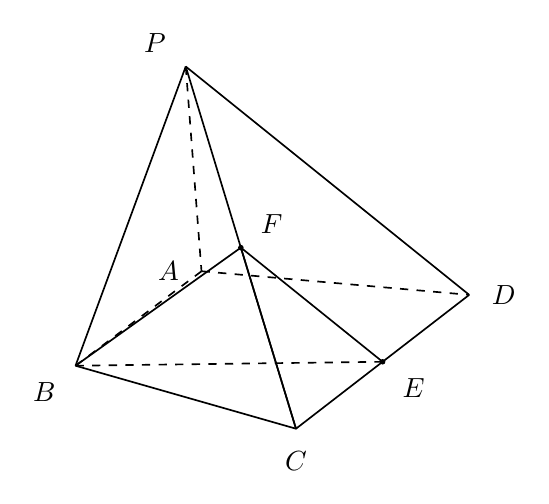
\begin{tikzpicture}[x=1cm,y=1cm,font=\normalsize,
  geometry edge/.style={solid,line width=.6pt,draw=black},
  geometry label/.style={font=\normalsize,inner sep=2pt}]

\coordinate (P) at (-0.2,3.6);
\coordinate (A) at (0,1.0);
\coordinate (B) at (-1.6,-0.2);
\coordinate (C) at (1.2,-1.0);
\coordinate (D) at (3.4,0.7);
\coordinate (E) at (2.3,-0.15);
\coordinate (F) at (0.5,1.3);
\draw[geometry edge] (P)--(B);
\draw[geometry edge] (P)--(D);
\draw[geometry edge] (P)--(C);
\draw[geometry edge] (B)--(C)--(D);
\draw[geometry edge] (B)--(F);
\draw[geometry edge] (F)--(E);
\draw[geometry edge] (F)--(C);
\draw[geometry edge,dashed] (P)--(A);
\draw[geometry edge,dashed] (A)--(B);
\draw[geometry edge,dashed] (A)--(D);
\draw[geometry edge,dashed] (B)--(E);
\fill (E) circle (1pt);
\fill (F) circle (1pt);
\node[geometry label,above left,xshift=-5pt,yshift=3pt] at (P) {$P$};
\node[geometry label,left,xshift=-6pt] at (A) {$A$};
\node[geometry label,below left,xshift=-5pt,yshift=-4pt] at (B) {$B$};
\node[geometry label,below,yshift=-6pt] at (C) {$C$};
\node[geometry label,right,xshift=6pt] at (D) {$D$};
\node[geometry label,below right,xshift=5pt,yshift=-4pt] at (E) {$E$};
\node[geometry label,above right,xshift=5pt,yshift=3pt] at (F) {$F$};
\end{tikzpicture}
